\autsubsection{Laser Drilling}{Bhaaeddin Alhomsi and Paul Connetable}

Lasers may provide another methodto dig through the layer of ice. High-power lasers exceeding 10 kW have been developed and widely used for industry (Gapontsev et al., 2009; Richardson et al., 2010; Fujita et al., 2010). For example, a recent laboratory test using a 1.6-kW pulsed Nd:YAG 1.064 $\mu$m wavelength laser beam determined the energy required to spall, melt, and
vaporize several rock samples for oil and gas well drilling. The required energy (specific energy) depends on the absorption properties of each rock sample as well as the reflective properties of the rock surface  (Gahan and Parker, 2001; Xu et al., 2003). A new laser-mechanical bit for laser spallation of rock to give an optimum drilling mechanism
was found to reduce rig time and increase drilling efficiency (Pooniwala, 2006).More recently, a 20-kWlaserwas delivered through a 1500 m-long optical fiber cable and shown to be able to efficiently drill oil and gas wells (Hecht, 2012). Finally, in the project VALKYRIE,
ice was drilled by a self-contained "intelligent ice penetrator", a 5 kW laser at 1070 nm wavelength (Siegel et al., 2013)(Stone et al., 2014).
Test of VALKYRIE between 2010 and 2013 used high-power optical energy transfer over km-scale distances and tested the feasibility of a vehicle deployed optical waveguide. Thus, a laser-drill system may be useful for ice-sheet applications, including the search for life in extreme environmental conditions here on Earth as well as outer planets.
With continual improvements, laser drilling may develop advantages over other methods for ice.We investigate here the behaviour of laser melting of ice and snow with an infrared laser for the potential use as a drill.


\subsubsection{Characteristics of light absorbance in ice}

The first step before selecting a laser is to analyze the spectral absorption of the medium we want to dig through. Therefore, the ice transmittance spectrum is displayed in Figure \ref{IceAbsorbance}. One can observe on this figure peaks of absorption, at around $10^{-5}~m$, and around $6\times10^{-5}~m$. The best suited lasers for digging through ice would have to emit at these frequencies.

Hence, we use a $CO_2$ laser, which is a relatively inexpensive common infrared gas laser (Patel, 1964) with fundamental lines from 9.2 to 10.8 $\mu$m and used in both pulse and continuous wave (CW) mode. For ice, an earlier study demonstrated the potential of $CO_2$ laser irradiation to help breakup nautical sea-ice (Clark et al.,  1973), but the laser has apparently not previously been used for snow and ice drilling.

\begin{figure}[htb]
\begin{center}
%\fbox{
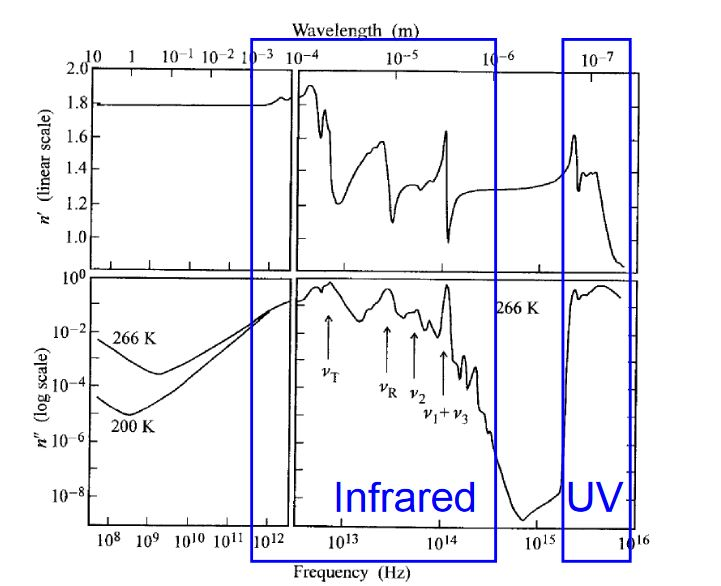
\includegraphics[width=16cm, clip]{figures/laser-drilling/iceabsorbance.JPG}
%}
\end{center}
\caption{Reported values of transmittance in ice}
\label{IceAbsorbance}
\end{figure}


The absorption of light in ice depends on the complex refractive index of ice. According to data in a previous study (Warren and Brandt, 2008), the absorption coefficient of ice significantly increases from the near- to mid-infra-red region, reaching a value of about $\unit[628.3]{cm^{-1}}$ at the $CO_2$ laser wavelength of 10.6 $\mu$m. Ice absorbs almost 100\% of the light intensity at 10.6 and 1.064 $\mu$m within a penetration distance of 0.01 and 2 cm, as shown in Figure \ref{fig:bh1}.

\begin{figure}[htb]
\centering
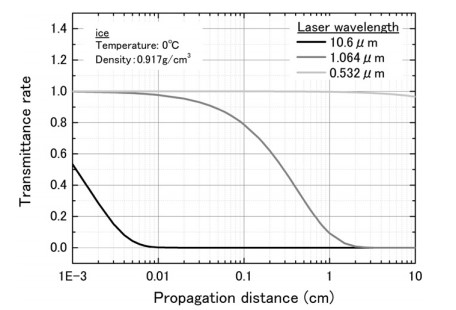
\includegraphics[scale=1]{figures/laser-drilling/bh1.jpg}
\caption{Characteristics of light absorbance in ice}
\label{fig:bh1}
\end{figure}

\subsubsection{Melting studies of ice and snow by $CO_2$ laser}

A $CO_2$ laser can be used to melt ice. The $CO_2$ laser at 10.6 $\mu$m (25.5 W) and a beam diameter of 1.0 cm, a wavelength at which ice strongly absorbs, to drill (via melting) through ice. The resulting drilling speed is measured at several irradiation intensities, ice-snow densities, and beam angles relative to the horizontal axis.
The melting speed increases with increasing laser intensity and with decreasing ice density, as shown in Figure \ref{fig:bh2}. The melting speed ratio between ice ($\unitfrac[917]{kg}{m^3}$) and the lowest-density snow ($\unitfrac[153]{kg}{m^3}$) is 4-5, slightly less than the value of \~6 expected from the density ratio. The reason for this discrepancy could be explained by the snow having a greater reflectivity than solid ice. The melting speed decreases with increasing snow density.

\begin{figure}[htb]
\centering
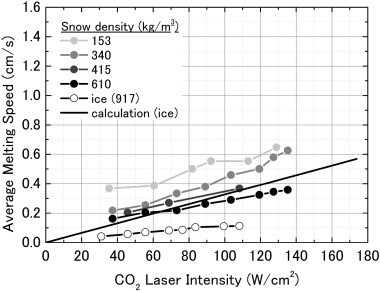
\includegraphics[scale=1]{figures/laser-drilling/bh2.jpg}
\caption{Relation between laser intensity and melting speed}
\label{fig:bh2}
\end{figure}

\subsubsection{Results}

Unfortunately, the experimental results indicate that the melt-water accumulates in the hole and reduces the melting speed of ice and a pump system could not be installed due to a high distance.
Moreover, since the energy source brought in the penetrator is a RTG, using a laser would require to transform the thermal energy produced by the RTG in electric energy. Such a conversion has an efficiency of about 20~\%. If we add to that the fact that the best $CO_{2}$ lasers also have efficiencies up to only 20~\%, the best efficiency achievable on this drilling method is of about 4~\%with the current technology. This is still while assuming that the ice absorbs all of the energy sent by the laser, which is not the case. It means that the efficiency of such a drilling method would be extremely low, and thus not indicated for our mission.
In future studies, it will be necessary to investigate quantitatively several additional factors. These include the optical-fiber coupled laser intensities required for deep drilling, and a method to pump melted water. Despite these hurdles, laser drilling is a promising technology for ice drilling. Lasers are indeed capable of delivering very high powers precisely. Furthermore, the main reason for low $CO_{2}$ lasers' efficiency is the power consumed for cooling the body of the laser. This efficiency could then go up if a laser specifically designed for our mission was done, since it could use the cold surroundings of the penetrator to cool down.